\subsection{Security Overview}

A computer system is said to be secure if it satisfies the following properties:
\begin{itemize}
\item {\bf Confidentiality}: Unauthorized entities cannot access the system or its data
\item {\bf Integrity}: When you receive data, it is the right one
\item {\bf Availability}: The system or data is there when you need it
\end{itemize}

\begin{rem}
The mere presence of these properties does not necessarily mean that the system is fully secure in practice.
\end{rem}

A secure system is reliable:

\begin{itemize}
    \item Keep your personal data confidential 
    \item Allow only authorised access or modifications to resources
    \item Ensure that any produced results are correct
    \item Give you correct and meaningful results whenever you want them
\end{itemize}


Terminology:

\begin{itemize}
    \item {\bf{Assets}}: Things we want to protect (hardware, software, data)
    \item {\bf{Vulnerabilities}}: Weaknesses in a system that may be exploited in order to cause loss and harm
    \item {\bf{Threats}}: A loss or harm that might befall a system (interception, interruption, modification, fabrication)
    \item {\bf{Attack}}: An action which exploits a vulnerability to execute a threat 
    \item {\bf{Control/Defence}}: Removing/reducing a vulnerability. You control a vulnerability to prevent an attack and defend against a threat
\end{itemize}

Methods of Defence:

\begin{itemize}
    \item Prevent it
    \item Deter it: make the attack harder or more expensive
    \item Deflect it: make yourself less attractive to attacker
    \item Detect it: notice that the attack is occurring
    \item Recover from it: mitigate the effects of the attack
\end{itemize}

Principle of Easiest Penetration: A system is only as secure as its weakest link. An attacker will go after whatever part of the system is easiest for them, not most convenient for you. In order to build secure systems, we need to learn how to think like an attacker!

\subsection{Defense Overview}
Software controls:
\begin{itemize}
    \item Passwords and other forms of access control
    \item Operating systems separate users' actions from each other
    \item Virus scanner watch for malware
    \item Development controls enforce quality measures on the original source code 
    \item Personal firewalls that run on your desktop
\end{itemize}

Hardware controls:
\begin{itemize}
    \item Not usually protection of the hardware itself, but rather using separate hardware to protect the system as a whole 
    \item Fingerprint readers
    \item Smart tokens
    \item Firewalls
    \item Intrusion detection systems
\end{itemize}

Physical Systems:
\begin{itemize}
    \item Protection of the hardwell itself, as well as physical access to the console, storage media, etc.
    \item Locks
    \item Guards
    \item Off-site backups
\end{itemize}

Policies and Procedures:
\begin{itemize}
    \item Non-technical means can be used to protect against some classes of attack (e.g. VPNs for accessing interal company network)
    \item Rules about choosing Passwords
    \item Training in best security practices
\end{itemize}

\subsection{Cryptography Overview}
Objectives of Cryptography:
\begin{itemize}
    \item Protecting data privacy
    \item Authenticaion (message, data origin, entity)
    \item Non-repudiation: preventing the sender from later denying that they sent the message
\end{itemize}

\begin{defn}
Kerkhoff's Principle: The adversary knows all details about a crypto system except the secret key.
\end{defn}

\begin{defn}
Cipher: A method or algorithm used to transform readable data (called plaintext) into an unreadable format (called ciphertext) to protect its confidentiality.
\end{defn}

Encryption is the process of converting plaintext into ciphertext. Decryption is the reverse process. Encryption uses the key k, decryption uses the key k'. If k = k', the system is symmetric. If k $\neq$ k', the system is asymmetric. Decryption(Encryption(m)) = m.
\begin{figure}[h!]
    \centering
    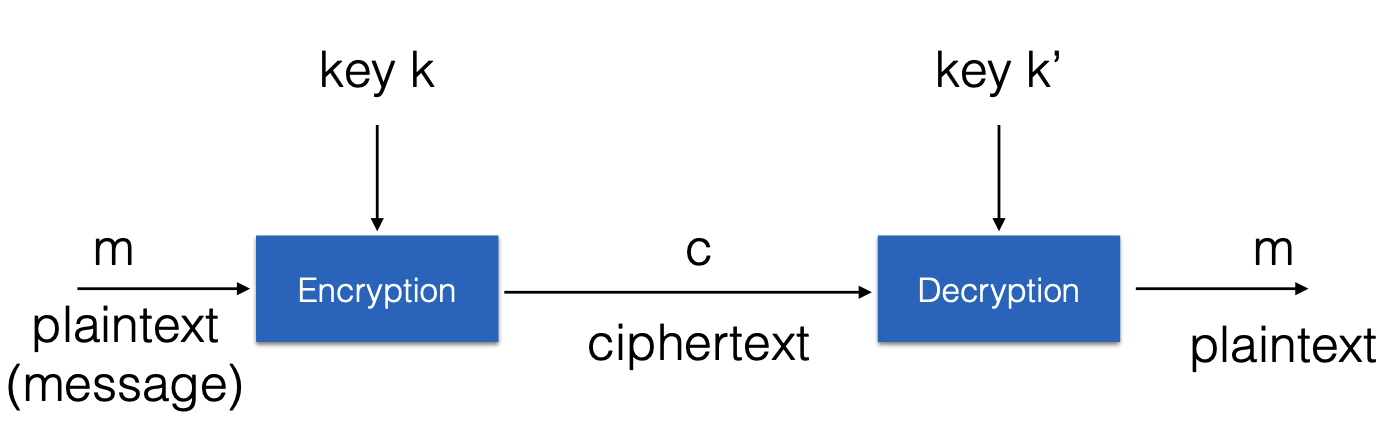
\includegraphics[scale=0.5]{img/w1encryption.png}
    \caption{Encryption}
\end{figure}

\begin{table}[h!]
    \centering
    \begin{tabular}{|l|l|l|}
    \hline
    \textbf{Feature}        & \textbf{Private Key Encryption}        & \textbf{Public Key Encryption}         \\ \hline
    \textbf{Keys}           & Same key for encryption \& decryption  & Two keys: public and private           \\ \hline
    \textbf{Speed}          & Faster                                 & Slower                                 \\ \hline
    \textbf{Key sharing}    & Must be kept secret                    & Only the private key is secret         \\ \hline
    \textbf{Use cases}      & Encrypting large data, e.g., files     & Secure key exchange, digital signatures \\ \hline
    \end{tabular}
    \caption{Summary of Differences Between Private and Public Key Encryption}
    \label{tab:encryption_comparison}
    \end{table}
    
\subsection{Topics Covered in Course}
\begin{itemize}
\item Classical systems: simple ciphers, substitution, permutation, transposition, Caesar, Vigenere
\item Information Theoretic Security
\item Defining security: pseudorandomness, one-way functions, trapdoor functions
\item Notions of security: perfect secrecy, semantic security, IND security
\item Attacks on encryption schemes: objective, levels of computing power, amount of information available
\item Types attacks: ciphertext-only, known plaintext, chosen plaintext, chosen ciphertext, adaptive
\item Different types of adversaries: unbounded/polynomial computing power
\item Security: unconditionally secure, computationally secure
\item and more... see slides
\end{itemize}
